\subsection{Language Models}
\label{sec:language_models}

\subsubsection{Statistical Machine Learning}

In statistical machine learning we need:
\begin{itemize}
    \item a \textbf{training corpus} $\mathcal{T}={(d_1,y_1),\dots,(d_m,y_m)}$.
    \item a \textbf{representation funciton} $\phi:D\rightarrow\mathbb{R}^n$, this
    function has to map each $d_i$ to it's corresponding $y_i$.
    \item to choose our \textbf{hypothesis class} $\mathcal{H}\in{f_1, f_2, \dots}$. It can be written like
    $f(\phi(d_i)|\Theta)=\hat{y_i}(\Theta)$. Where $\Theta$ are the parameters
    of the model. We usually chose an arbitrary hypothesis class and then we
    check if its output is good enough.
    \item an \textbf{error function} $\mathcal{L}(\Theta)=\sum_i e(y_i,\hat{y_i})$.
    \item to find a value of $\Theta$ to minimize $\mathcal{L}$.
\end{itemize}

\subsubsection{Definitions}

\begin{itemize}
    \item \textbf{Vocabulary}: a finite set of something, denoted as $V$.
    The elements that we will denote as $w\in V$ are called \textbf{words}.
    \item \textbf{Sentence}: a sequence of $n$ words in $V$ denoted as $s=w_1,\dots,w_n$.
    We denote with $V^+$ the infinite set (but numerable) of all finite sentences over 
    $V$ (not necessarily grammatically correct).
    \item \textbf{Language model}: a language model over $V^+$ is a function $P:V^+\rightarrow\mathbb{R}$
    s.t. $\forall s\in V^+$ we have $P[s]\geq 0$ and $\sum_{s\in V^+}P[s]=1$. This is a probability distribution
    over $V^+$.
\end{itemize}

From now on $P[s]$ is a number $\in[0,1]$ while $P(s)$ is a probability distribution where $s$ denotes a random variable
over $V^+$. We will also uso $P[w]$ and $P(w)$ to denote the same thing as before but with single word sentences.

$V^+$ is infinite so we cannot store it, we have to approximate it with $\mathcal{T}$.
\begin{figure}[H]
    \centering
    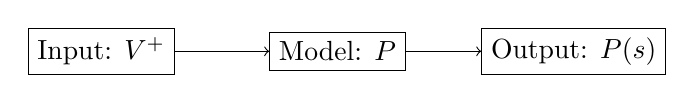
\begin{tikzpicture}
        \node (input) [draw, rectangle] {Input: $V^+$};
        \node (model) [draw, rectangle, right of=input, node distance=3cm] {Model: $P$};
        \node (output) [draw, rectangle, right of=model, node distance=3cm] {Output: $P(s)$};
        
        \draw[->] (input) -- (model);
        \draw[->] (model) -- (output);
    \end{tikzpicture}
    \caption{The ideal model.}
    \label{fig:language_model}
\end{figure}

\begin{figure}[H]
    \centering
    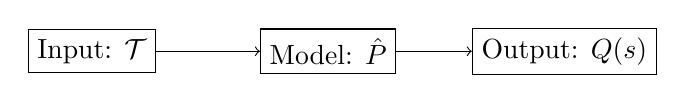
\begin{tikzpicture}
        \node (input) [draw, rectangle] {Input: $\mathcal{T}$};
        \node (model) [draw, rectangle, right of=input, node distance=3cm] {Model: $\hat{P}$};
        \node (output) [draw, rectangle, right of=model, node distance=3cm] {Output: $Q(s)$};
        
        \draw[->] (input) -- (model);
        \draw[->] (model) -- (output);
    \end{tikzpicture}
    \caption{The approximate model.}
    \label{fig:approximated_language_model}
\end{figure}

A vocabulary can contain all possible words in a language
but it can also have some missing, in that case we add a special word $<OOV>$ to represent
all the words that are not in the vocabulary.

How close is $Q(s)$ to $P(s)$?

If we use the model for a \textbf{downstream task} we need to evaluate the model on the specific task that
it will be used for.

To evaluate a model in general we need an evaluation corpus $\mathcal{E}$ that is
still a subset of $V^+$ and has a very small intersection with $\mathcal{T}$.

Let's say that an evaluation corpus is composed of $n$ sentences $s_1,\dots,s_n$.
We concatenate all the sentences to form a single huge sentence $w_1,\dots,w_T$.
The \textbf{perplexity} of the model $P$ over $w_1,\dots,w_T$ is defined as:
\[
    PP(w_1,\dots,w_T)=P[w_1,\dots,w_T]^{-\frac{1}{T}}
\]
\[
    P[w_1,\dots,w_T]=P[w_1]\prod_{i=2}^{T}P[w_i|w_1,\dots,w_{i-1}]
\]
\[
    PP(w_1,\dots,w_T)=\left(P[w_1]\prod_{i=2}^{T}P[w_i|w_1,\dots,w_{i-1}]\right)^{-\frac{1}{T}}
\]

This is the \textbf{geometric mean} of the inverse of the probability of each word in the sentence.

What is $P[w_i|w_1,\dots,w_{i-1}]$? It's the probability of seeing
the word $w_i$ given the previous part of the sentence.

The perplexity measures how overall the number of choices has been reduced
while generating the sentence. How many words on average are
probable (with non 0 probability) given a starting sentence.

In English the perplexity is tought to be arount 15 and 20.

If we consider the \textbf{uniform language model} where $P[w_i|w_1,\dots,w_{i-1}]=\frac{1}{|V|}$ 
(the words are all equally probable and independent) we have:
\[
    P[w_1,\dots,w_T]=\left(\frac{1}{|V|}\right)^T
\]
\[
    PP(w_1,\dots,w_T)=|V|
\]
This makes sense as we randomly choose a word from $V$ at each step.

We have to mark the start and the end of the sentence with special words $<s>$ and $</s>$.
To take this into account we would have to modify the perplexity formula (would be a bit nicer).
These two words are ignored for the rest of the notes.

At this point we can use a model to generate a sentence.

Given a starting sentence $w_1,\dots,w_n$ we want to generate $\hat{w_1},\dots,\hat{w_m}$.
We can find $\hat{w_1}$ as $\hat{w_1}=\text{argmax}_{w\in V}P[w|w_1,\dots,w_n]$.
Then we can append $\hat{w_1}$ to the sentence and repeat the process until we reach the end of the sentence.
This is called \textbf{greedy search}.
